\chapter{Modelagem de assentamento de dutos submarinos}
\label{chap:assentamento}


O assentamento de dutos submarinos tem sido o núcleo da engenharia \textit{offshore} por meio século.
Vários métodos e técnicas tem sido desenvolvidas e usadas para dutos submarinos~\cite{Ivic2016}.
O processo de lançamento de dutos é uma das tarefas mais desafiadoras, mesmo quando a rota ideal já está definida.
Modelar a instalação de dutos em um \textit{software} de elementos finitos para uso geral pode ser um trabalho demorado e tedioso, principalmente devido a grandes quantidades de dados da batimetria.
Na maioria das vezes, são necessárias técnicas avançadas de \textit{script} para definir o perfil do leito marinho, selecionar a rota ideal do duto e simular o processo de assentamento~\cite{VandenAbeele2013}.

A simulação do duto projetado em um ambiente tridimensional realista obtido por medições da topografia do fundo marinho, permite que os engenheiros explorem quaisquer oportunidades que o comportamento do mesmo pode oferecer para desenvolver soluções seguras e econômicas.
Por exemplo, o projetista pode analisar primeiro o comportamento do duto na batimetria original.
Se alguns dos casos de carga resultam em tensões além do limite aceitável, pode-se simular uma modificação do fundo do mar no modelo de elementos finitos.
A análise é então executada novamente para confirmar que as modificações levaram à diminuição desejada de tensão ou deformação.

O modelo de elementos finitos pode ser uma ferramenta para analisar o comportamento \textit{in-situ} de um duto.
Por comportamento \textit{in-situ} duto entenda-se a resposta do mesmo as cargas ao longo de parte do todo o seu histórico de carregamento~\cite{Bai2014}, isso pode consistir em vários casos de carga em sequência, por exemplo:

\begin{enumerate}
    \item instalação;
    \item testes de pressão (enchimento de água e do teste hidrostático);
    \item operação (enchimento com conteúdo, pressão de projeto e temperatura);
    \item ciclos de carga/descarga;
    \item flambagem lateral e vertical (\textit{upheaval});
    \item onda dinâmica e/ou de corrente;
    \item cargas de impacto.
\end{enumerate}

\section{Modelagem do sistema de dutos com Elementos Finitos}

A modelagem da instalação do duto é o primeiro passo para o estudo do comportamento \textit{in-situ} do duto, e visa reproduzir a configuração indeformada do duto assim que lançado sobre a leito marinho.
Esta configuração serve como ponto de partida para as etapas posteriores da análise.
Mais importante do que investigar o comportamento do duto durante a instalação é garantir que a correta representação da tração e ângulo de lançamento de tal modo que consigam gerar forças residuais no duto, oriundas do atrito quando o duto se assenta sobre a batimetria.

\begin{figure}[th!]
    \centering
    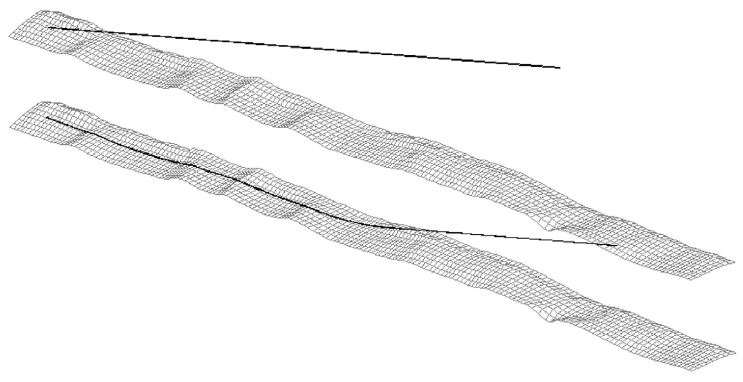
\includegraphics[width=0.7\linewidth]{imagens/lancamento_do_duto}
    \caption[Modelo de elementos finitos durante o lançamento]{Modelo de elementos finitos durante o lançamento.\\Fonte:~\cite{Bai2014}}\label{fig:lancamentododuto}
\end{figure}

Por simplicidade, neste trabalho, vamos assumir que o ângulo entre o duto e a horizontal o será nulo, isto é, o duto estará num plano horizontal que desce em direção a superfície batimétrica.
Desso modo, o modelo permitirá especificar somente a tração de lançamento.
Essa modelagem visa garantir a correta representação do contato entre o duto e a batimetria (forças de contato e ponto onde o duto toca o solo).
A Figura~\ref{fig:lancamentododuto} mostra o duto antes e durante o processo de instalação.

A medida que o duto se assenta é necessário garantir um equilíbrio estável entre o duto e o solo, o que é feito mediante um modelo representativo dessa iteração, no qual deve-se definir o atrito e rigidez do leito marinho.
No Abaqus~\cite{Simulia2018}, pode-ser relacionar a penetração e a pressão de resposta do solo por meio de uma curva de rigidez axial, além de usar modelo anisotrópico para o atrito do solo para representar as diferenças entre os atritos nas direções longitudinal e transversal.
